% Options for packages loaded elsewhere
\PassOptionsToPackage{unicode}{hyperref}
\PassOptionsToPackage{hyphens}{url}
\PassOptionsToPackage{dvipsnames,svgnames,x11names}{xcolor}
%
\documentclass[
  letterpaper,
  DIV=11,
  numbers=noendperiod]{scrartcl}

\usepackage{amsmath,amssymb}
\usepackage{iftex}
\ifPDFTeX
  \usepackage[T1]{fontenc}
  \usepackage[utf8]{inputenc}
  \usepackage{textcomp} % provide euro and other symbols
\else % if luatex or xetex
  \usepackage{unicode-math}
  \defaultfontfeatures{Scale=MatchLowercase}
  \defaultfontfeatures[\rmfamily]{Ligatures=TeX,Scale=1}
\fi
\usepackage{lmodern}
\ifPDFTeX\else  
    % xetex/luatex font selection
\fi
% Use upquote if available, for straight quotes in verbatim environments
\IfFileExists{upquote.sty}{\usepackage{upquote}}{}
\IfFileExists{microtype.sty}{% use microtype if available
  \usepackage[]{microtype}
  \UseMicrotypeSet[protrusion]{basicmath} % disable protrusion for tt fonts
}{}
\makeatletter
\@ifundefined{KOMAClassName}{% if non-KOMA class
  \IfFileExists{parskip.sty}{%
    \usepackage{parskip}
  }{% else
    \setlength{\parindent}{0pt}
    \setlength{\parskip}{6pt plus 2pt minus 1pt}}
}{% if KOMA class
  \KOMAoptions{parskip=half}}
\makeatother
\usepackage{xcolor}
\setlength{\emergencystretch}{3em} % prevent overfull lines
\setcounter{secnumdepth}{-\maxdimen} % remove section numbering
% Make \paragraph and \subparagraph free-standing
\ifx\paragraph\undefined\else
  \let\oldparagraph\paragraph
  \renewcommand{\paragraph}[1]{\oldparagraph{#1}\mbox{}}
\fi
\ifx\subparagraph\undefined\else
  \let\oldsubparagraph\subparagraph
  \renewcommand{\subparagraph}[1]{\oldsubparagraph{#1}\mbox{}}
\fi


\providecommand{\tightlist}{%
  \setlength{\itemsep}{0pt}\setlength{\parskip}{0pt}}\usepackage{longtable,booktabs,array}
\usepackage{calc} % for calculating minipage widths
% Correct order of tables after \paragraph or \subparagraph
\usepackage{etoolbox}
\makeatletter
\patchcmd\longtable{\par}{\if@noskipsec\mbox{}\fi\par}{}{}
\makeatother
% Allow footnotes in longtable head/foot
\IfFileExists{footnotehyper.sty}{\usepackage{footnotehyper}}{\usepackage{footnote}}
\makesavenoteenv{longtable}
\usepackage{graphicx}
\makeatletter
\def\maxwidth{\ifdim\Gin@nat@width>\linewidth\linewidth\else\Gin@nat@width\fi}
\def\maxheight{\ifdim\Gin@nat@height>\textheight\textheight\else\Gin@nat@height\fi}
\makeatother
% Scale images if necessary, so that they will not overflow the page
% margins by default, and it is still possible to overwrite the defaults
% using explicit options in \includegraphics[width, height, ...]{}
\setkeys{Gin}{width=\maxwidth,height=\maxheight,keepaspectratio}
% Set default figure placement to htbp
\makeatletter
\def\fps@figure{htbp}
\makeatother
% definitions for citeproc citations
\NewDocumentCommand\citeproctext{}{}
\NewDocumentCommand\citeproc{mm}{%
  \begingroup\def\citeproctext{#2}\cite{#1}\endgroup}
\makeatletter
 % allow citations to break across lines
 \let\@cite@ofmt\@firstofone
 % avoid brackets around text for \cite:
 \def\@biblabel#1{}
 \def\@cite#1#2{{#1\if@tempswa , #2\fi}}
\makeatother
\newlength{\cslhangindent}
\setlength{\cslhangindent}{1.5em}
\newlength{\csllabelwidth}
\setlength{\csllabelwidth}{3em}
\newenvironment{CSLReferences}[2] % #1 hanging-indent, #2 entry-spacing
 {\begin{list}{}{%
  \setlength{\itemindent}{0pt}
  \setlength{\leftmargin}{0pt}
  \setlength{\parsep}{0pt}
  % turn on hanging indent if param 1 is 1
  \ifodd #1
   \setlength{\leftmargin}{\cslhangindent}
   \setlength{\itemindent}{-1\cslhangindent}
  \fi
  % set entry spacing
  \setlength{\itemsep}{#2\baselineskip}}}
 {\end{list}}
\usepackage{calc}
\newcommand{\CSLBlock}[1]{\hfill\break\parbox[t]{\linewidth}{\strut\ignorespaces#1\strut}}
\newcommand{\CSLLeftMargin}[1]{\parbox[t]{\csllabelwidth}{\strut#1\strut}}
\newcommand{\CSLRightInline}[1]{\parbox[t]{\linewidth - \csllabelwidth}{\strut#1\strut}}
\newcommand{\CSLIndent}[1]{\hspace{\cslhangindent}#1}

\KOMAoption{captions}{tableheading}
\makeatletter
\@ifpackageloaded{caption}{}{\usepackage{caption}}
\AtBeginDocument{%
\ifdefined\contentsname
  \renewcommand*\contentsname{Table of contents}
\else
  \newcommand\contentsname{Table of contents}
\fi
\ifdefined\listfigurename
  \renewcommand*\listfigurename{List of Figures}
\else
  \newcommand\listfigurename{List of Figures}
\fi
\ifdefined\listtablename
  \renewcommand*\listtablename{List of Tables}
\else
  \newcommand\listtablename{List of Tables}
\fi
\ifdefined\figurename
  \renewcommand*\figurename{Figure}
\else
  \newcommand\figurename{Figure}
\fi
\ifdefined\tablename
  \renewcommand*\tablename{Table}
\else
  \newcommand\tablename{Table}
\fi
}
\@ifpackageloaded{float}{}{\usepackage{float}}
\floatstyle{ruled}
\@ifundefined{c@chapter}{\newfloat{codelisting}{h}{lop}}{\newfloat{codelisting}{h}{lop}[chapter]}
\floatname{codelisting}{Listing}
\newcommand*\listoflistings{\listof{codelisting}{List of Listings}}
\makeatother
\makeatletter
\makeatother
\makeatletter
\@ifpackageloaded{caption}{}{\usepackage{caption}}
\@ifpackageloaded{subcaption}{}{\usepackage{subcaption}}
\makeatother
\ifLuaTeX
  \usepackage{selnolig}  % disable illegal ligatures
\fi
\usepackage{bookmark}

\IfFileExists{xurl.sty}{\usepackage{xurl}}{} % add URL line breaks if available
\urlstyle{same} % disable monospaced font for URLs
\hypersetup{
  pdftitle={DSCI 310 Group 8: Online Shopper},
  pdfauthor={Calvin Choi, Nour Abdelfattah, Sai Pusuluri, Sana Shams},
  colorlinks=true,
  linkcolor={blue},
  filecolor={Maroon},
  citecolor={Blue},
  urlcolor={Blue},
  pdfcreator={LaTeX via pandoc}}

\title{DSCI 310 Group 8: Online Shopper}
\author{Calvin Choi, Nour Abdelfattah, Sai Pusuluri, Sana Shams}
\date{}

\begin{document}
\maketitle

\renewcommand*\contentsname{Table of contents}
{
\hypersetup{linkcolor=}
\setcounter{tocdepth}{2}
\tableofcontents
}
\subsection{Summary}\label{summary}

E-commerce pages host several customers at any given moment, yet its
metric of success lies in the visitors who ultimately make purchase.
This project uses several machine learning models to learn from webpage
data and customer browsing behaviour in order to predict whether or not
a given customer will finalize their purchase.

\subsection{Introduction}\label{introduction}

It has been no surprise that retail giants like Walmart and Ikea have
aggressively invested and developed their e-commerce experiences
transitioning away from big box store fronts and converting those assets
to hubs for location-based fulfillment Monteros (2023). The
post-pandemic affects on consumer behaviour have accelerated our
dependency on digital platforms and have pushed the e-commerce industry
to grow a whopping 25\% to an industry worth over \$4 trillion USD Shaw,
Eschenbrenner, and Baier (2022). Consequently, online storefronts get a
lot of site traffic but what ultimately matters is their decision to
purchase and the volume of revenue. Marketing and User Experience teams
are tasked with optimizing a site's interface and content in order to
improve customer retention and the site's revenue. Given this,
understanding customer browsing behaviour and web page features is
crucial for not only improving the user's experience, but also
maximizing the retailer's revenue. Traditionally marketing and user
experience studies are conducted through surveys, interviews and
ethnographic studies, taking weeks up to months to process. However,
machine learning-based marketing research has exponentially reduced the
rate at which web metrics and purchase conversion strategies can be
processed, while significantly increasing purchase prediction accuracy
Gkikas and Theodoridis (2022). A common method to evaluate user
retention for online web browsing is through clickstream data of the
user's navigation path, however Saka et al.~found that combining this
information with session information significantly improves the purchase
success rate Sakar et al. (2018).

This project aims to analyze various features of online shopper's
sessions on a site to predict whether the customer makes a purchase. We
will use the dataset,
\href{https://archive.ics.uci.edu/dataset/468/online+shoppers+purchasing+intention+dataset}{Online
Shoppers Purchasing Intention} dataset from the UCI Machine Learning
Repository. This dataset was chosen specifically due to its coverage of
both user navigation data and session information, allowing for a
well-rounded analysis of both the user and e-commerce page's profile.

\textbf{Question}

Using all variables provided in the dataset, which group of explanatory
variables form the best prediction for the user's purchase intent?

\subsection{Exploratory Data Analysis}\label{exploratory-data-analysis}

Before starting our analysis, we will perform exploratory data analysis
in order to have a better understanding of the distributions of the
features in our dataset, as well as their contribution to our target
feature, Revenue.

The dataset provides the following features:

\paragraph{Summary of features}\label{summary-of-features}

\begin{itemize}
\tightlist
\item
  \textbf{Administrative}: the number of pages visited by user of this
  administrative type
\item
  \textbf{Administrative\_Duration}: the amount of time spent on pages
  of this administrative type
\item
  \textbf{Informational}: the number of pages visited by user of this
  informational type
\item
  \textbf{Informational\_Duration}: the amount of time spent on this
  informational category of pages
\item
  \textbf{ProductRelated}: the number of pages of this type of product
  the user visited
\item
  \textbf{ProductRelated\_Duration}: the amount of time spent on pages
  featuring related products
\item
  \textbf{BounceRates}: percentage of visitors who enter the web page
  then leave (``bounce'') without triggering any other requests to the
  analytics server during the session
\item
  \textbf{ExitRates}: the percentage of pageviews where the given page
  is the last page before exiting website
\item
  \textbf{PageValues}: the average value for a web page that a user
  visited before completing an e-commerce transaction
\item
  \textbf{SpecialDay}: the temporal proximity between the day the user
  is visiting the page and a special day (eg. Valentines Day, Christmas,
  Mother's Day, etc.).
\item
  \textbf{Month}: the month the page was viewed
\item
  \textbf{OperatingSystems}: an integer value representing the operating
  system of the user when viewing the page
\item
  \textbf{Browser}: an integer value representing the user's browser
  when viewing the page
\item
  \textbf{Region}: an integer value representing the user's traffic
  type.
  \href{https://www.practicalecommerce.com/Understanding-Traffic-Sources-in-Google-Analytics}{Learn
  more about user traffic types here}
\item
  \textbf{VisitorType}: categorizes the user into `New Visitor',
  `Returning Visitor', and `Other'.
\item
  \textbf{Weekend}: a boolean value, indicating whether the user's
  session took place during a weekend or not
\item
  \textbf{Revenue}: a boolean value, indicating whether the user made
  the purchase or not

  \begin{itemize}
  \tightlist
  \item
    \textbf{This will be our target feature}
  \end{itemize}
\end{itemize}

\paragraph{Exploratory Visualization}\label{exploratory-visualization}

To inform the chosen method of visualization, let us first document if
the features are continuous values, or if they are discrete categorical
values. Some features are categorical but represented as integers so
this step will allow for clarification.

\begin{longtable}[]{@{}ll@{}}
\caption{Data Types Summary}\label{tbl-features}\tabularnewline
\toprule\noalign{}
Feature & Type \\
\midrule\noalign{}
\endfirsthead
\toprule\noalign{}
Feature & Type \\
\midrule\noalign{}
\endhead
\bottomrule\noalign{}
\endlastfoot
Administrative & numerical, continuous \\
Administrative\_Duration & numerical, continuous \\
Informational & numerical, continuous \\
Informational\_Duration & numerical, continuous \\
ProductRelated & numerical, continuous \\
ProductRelated\_Duration & numerical, continuous \\
BounceRates & numerical, continuous \\
ExitRates & numerical, continuous \\
PageValues & numerical, continuous \\
SpecialDay & numerical, continuous \\
Month & categorical, discrete \\
Browser & categorical, discrete \\
Region & categorical, discrete \\
TrafficType & categorical, discrete \\
VisitorType & categorical, discrete \\
Weekend & categorical, discrete, boolean \\
Revenue & categorical, discrete, boolean \\
\end{longtable}

The summary of each datatype is provided in Table~\ref{tbl-features}

Given that Revenue is our target feature, let us examine its
distribution in Figure~\ref{fig-revenue-distribution}.

\begin{figure}[H]

\centering{

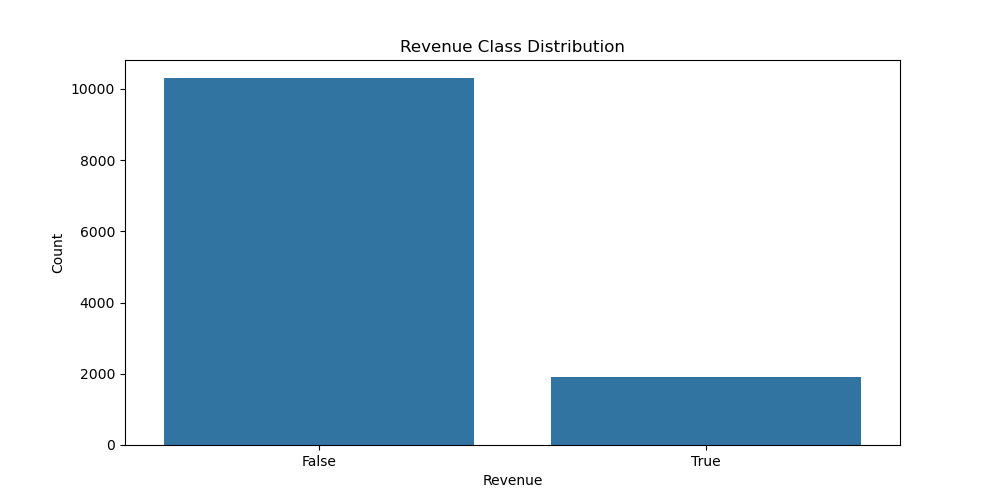
\includegraphics[width=0.8\textwidth,height=\textheight]{../results/figure_revenue_class_distribution.png}

}

\caption{\label{fig-revenue-distribution}Revenue Class Distribution}

\end{figure}%

Figure 2 shows that there does seem to be some class imbalance in the
Revenue feature. This might create bias in our models that may perform
poorly on the `True' Revenue cases as there were less examples to fit
on.

To compare Revenue with other features, we will perform some feature
engineering by creating the feature, Total Revenue, for each of the
categorical revenues explored below.

\paragraph{Categorical Features: Examining the
Distributions}\label{categorical-features-examining-the-distributions}

Let us examine the distribution of certain categorical feature to better
understand the user demographic.The distributions are:

\begin{itemize}
\item
  distribution of classes within the categorical feature
\item
  distribution of Revenue=True across the different classes for a given
  feature
\end{itemize}

\begin{figure}[H]

\centering{

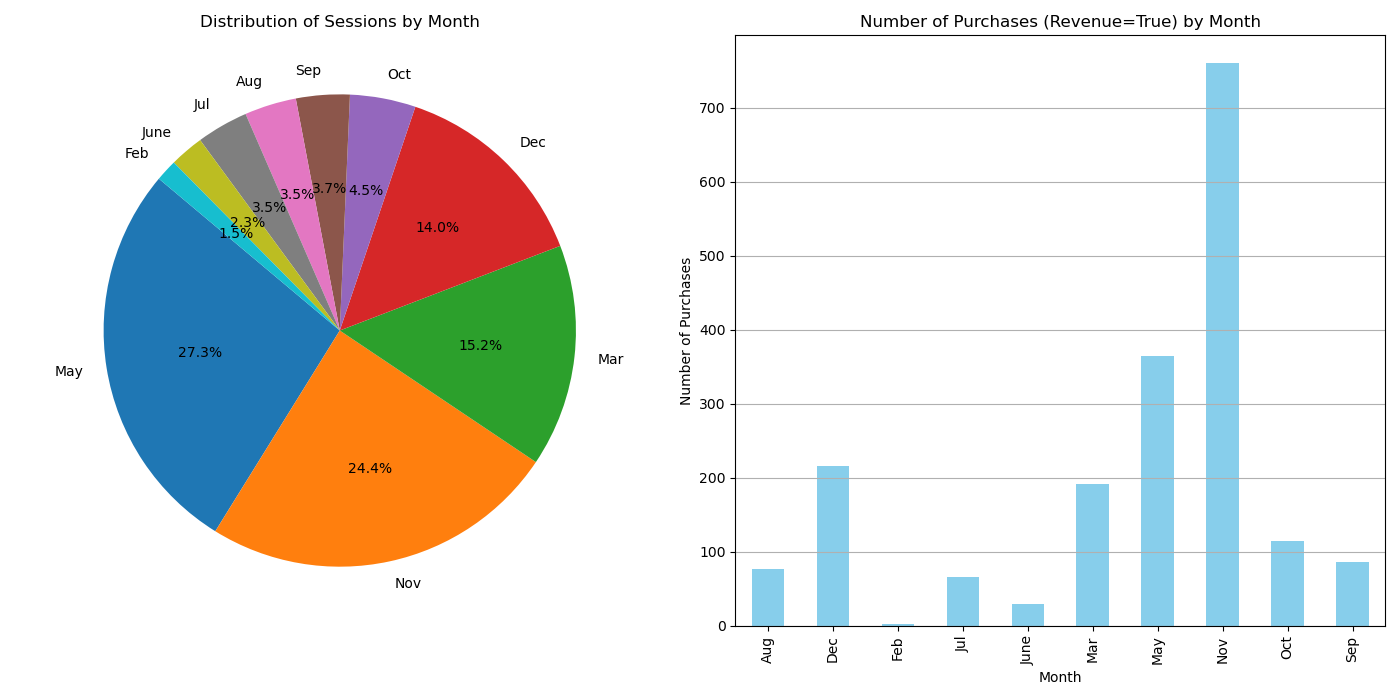
\includegraphics[width=0.8\textwidth,height=\textheight]{../results/figure_month_distribution.png}

}

\caption{\label{fig-month-distribution}Distribution of Sessions by
Month}

\end{figure}%

\begin{figure}[H]

\centering{

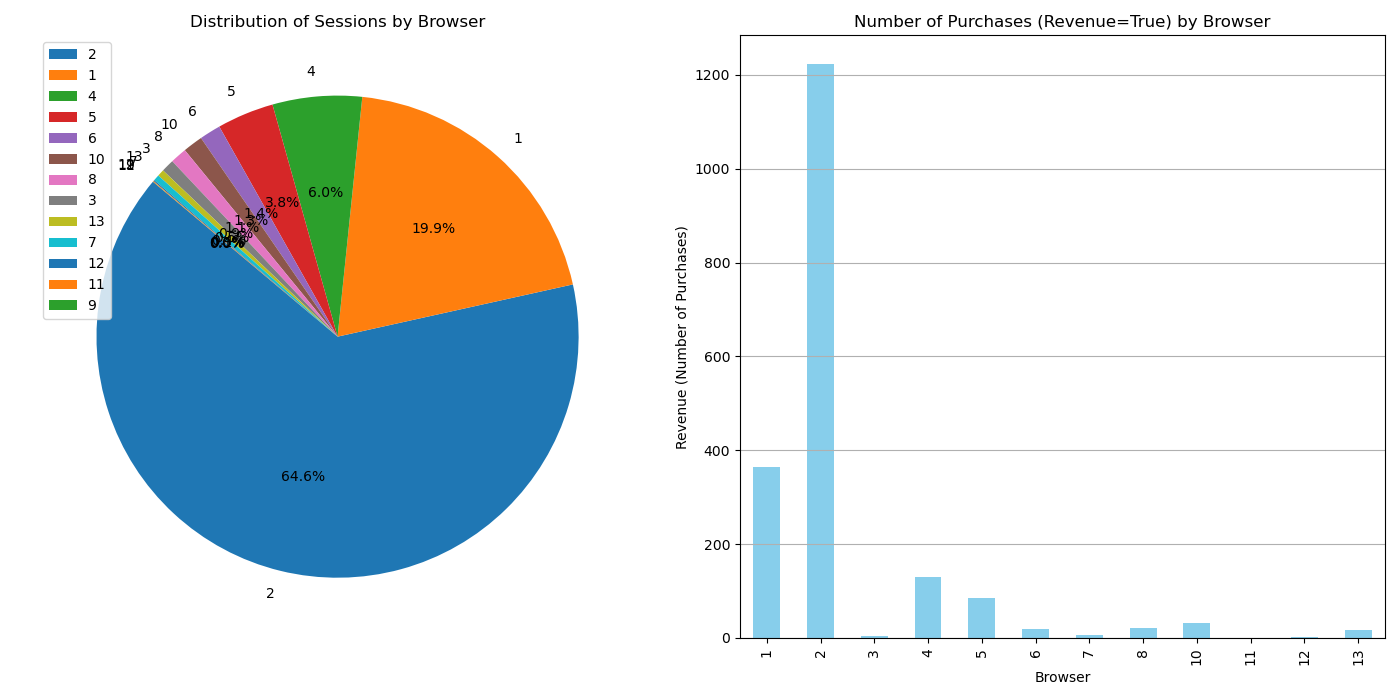
\includegraphics[width=0.8\textwidth,height=\textheight]{../results/figure_browser_distribution.png}

}

\caption{\label{fig-month-distribution}Distribution of Sessions by
Browser}

\end{figure}%

\begin{figure}[H]

\centering{

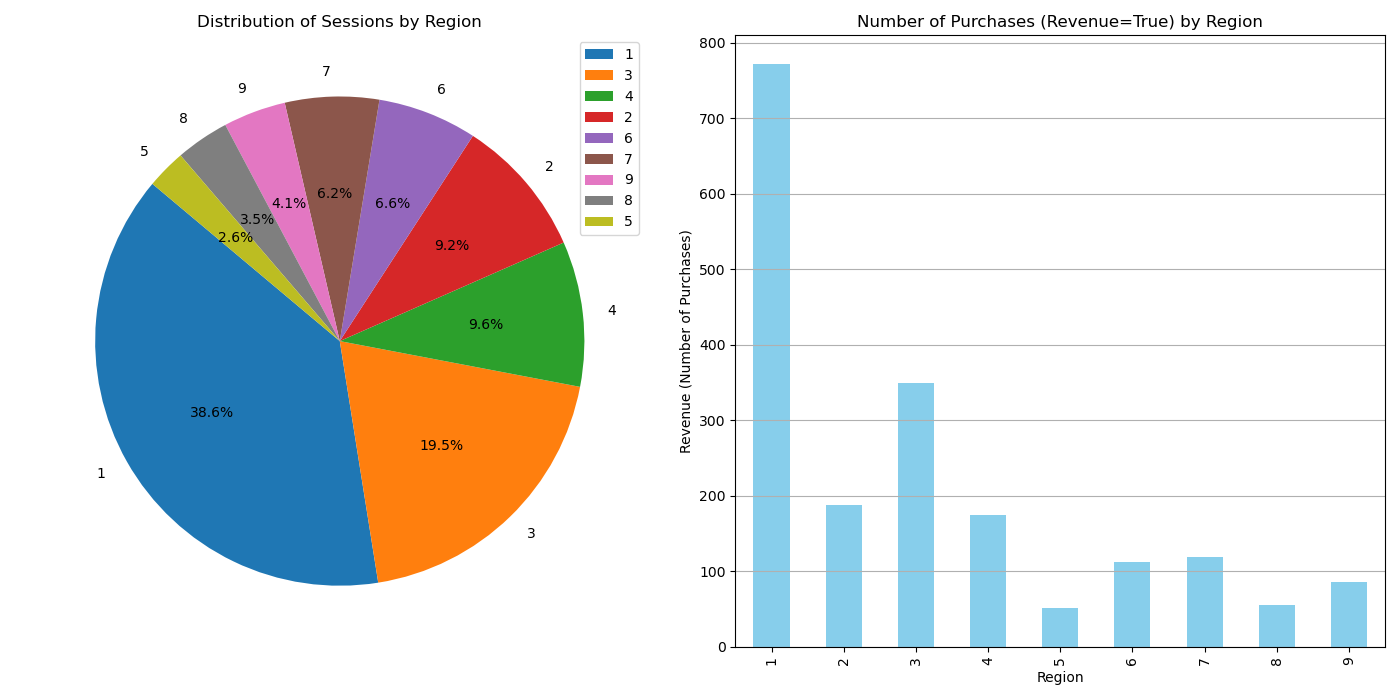
\includegraphics[width=0.8\textwidth,height=\textheight]{../results/figure_region_distribution.png}

}

\caption{\label{fig-region-distribution}Distribution of Sessions by
Region}

\end{figure}%

\begin{figure}[H]

\centering{

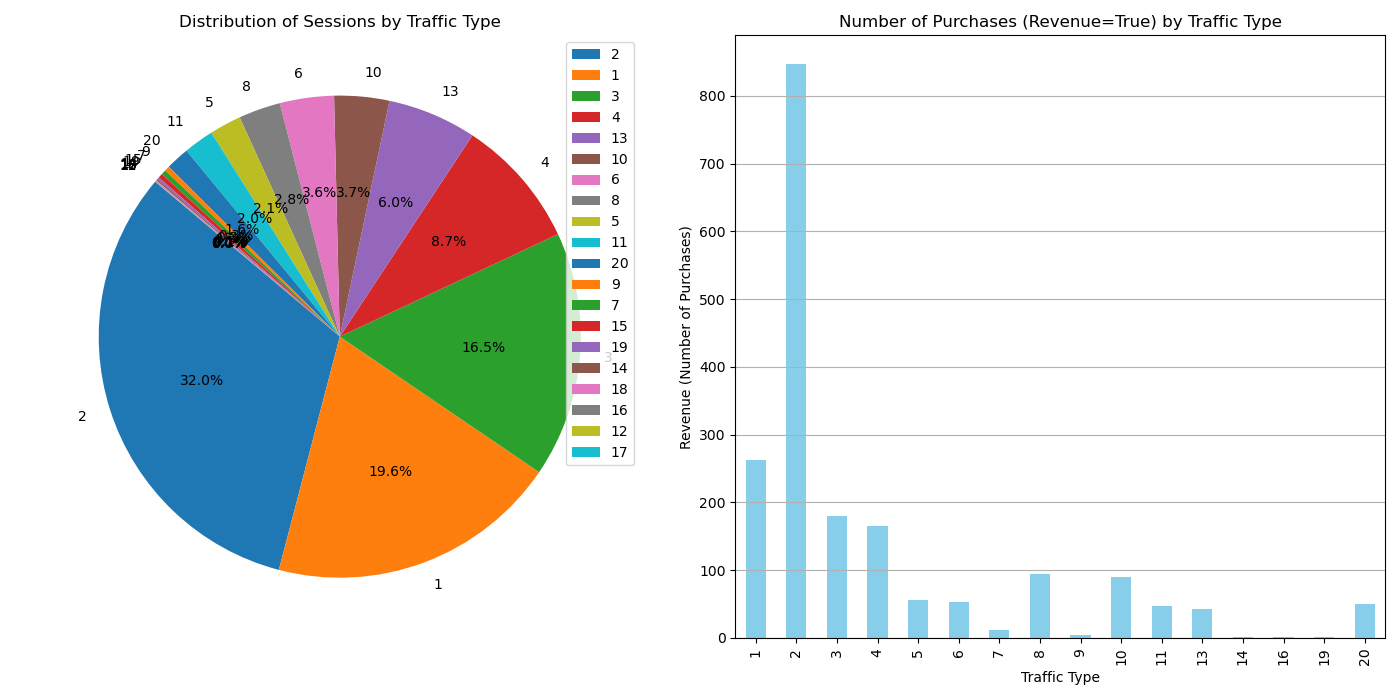
\includegraphics[width=0.8\textwidth,height=\textheight]{../results/figure_traffic_type_distribution.png}

}

\caption{\label{fig-traffic-distribution}Distribution of Sessions by
Traffic Type}

\end{figure}%

\begin{figure}[H]

\centering{

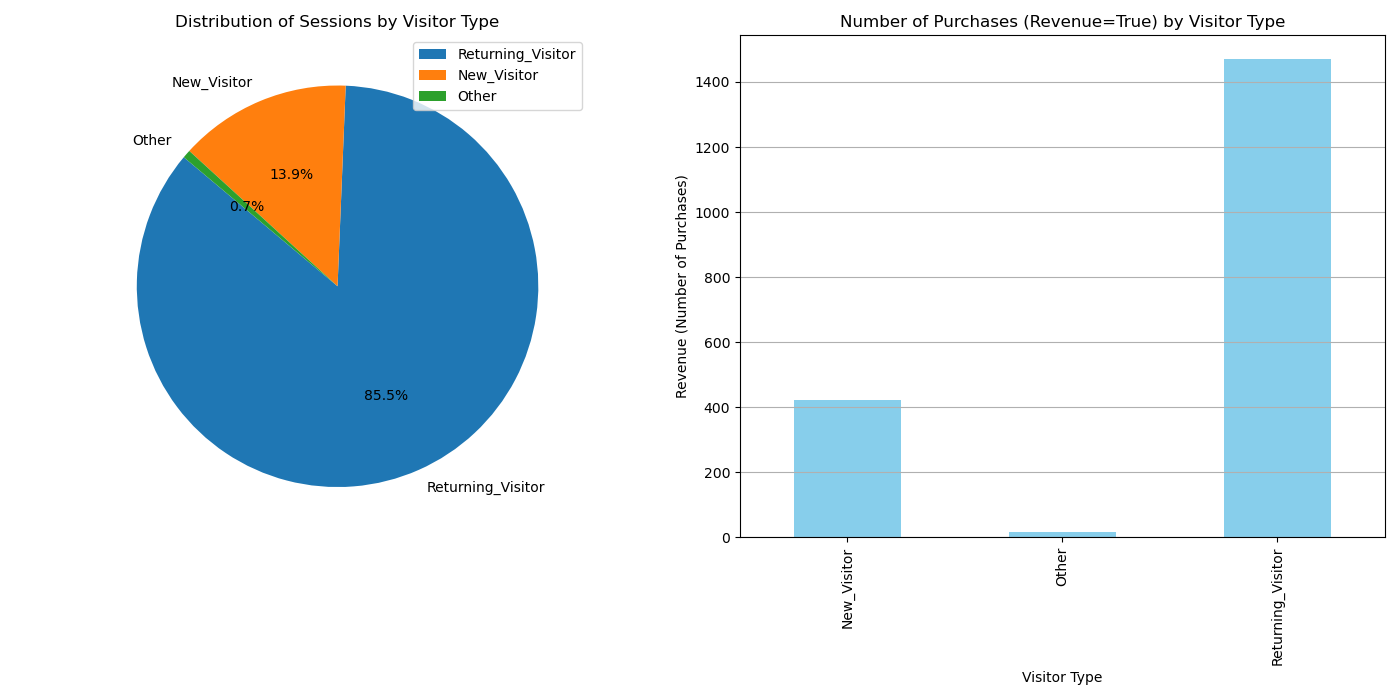
\includegraphics[width=0.8\textwidth,height=\textheight]{../results/figure_visitor_type_distribution.png}

}

\caption{\label{fig-visitor-distribution}Distribution of Sessions by
Visitor Type}

\end{figure}%

\begin{figure}[H]

\centering{

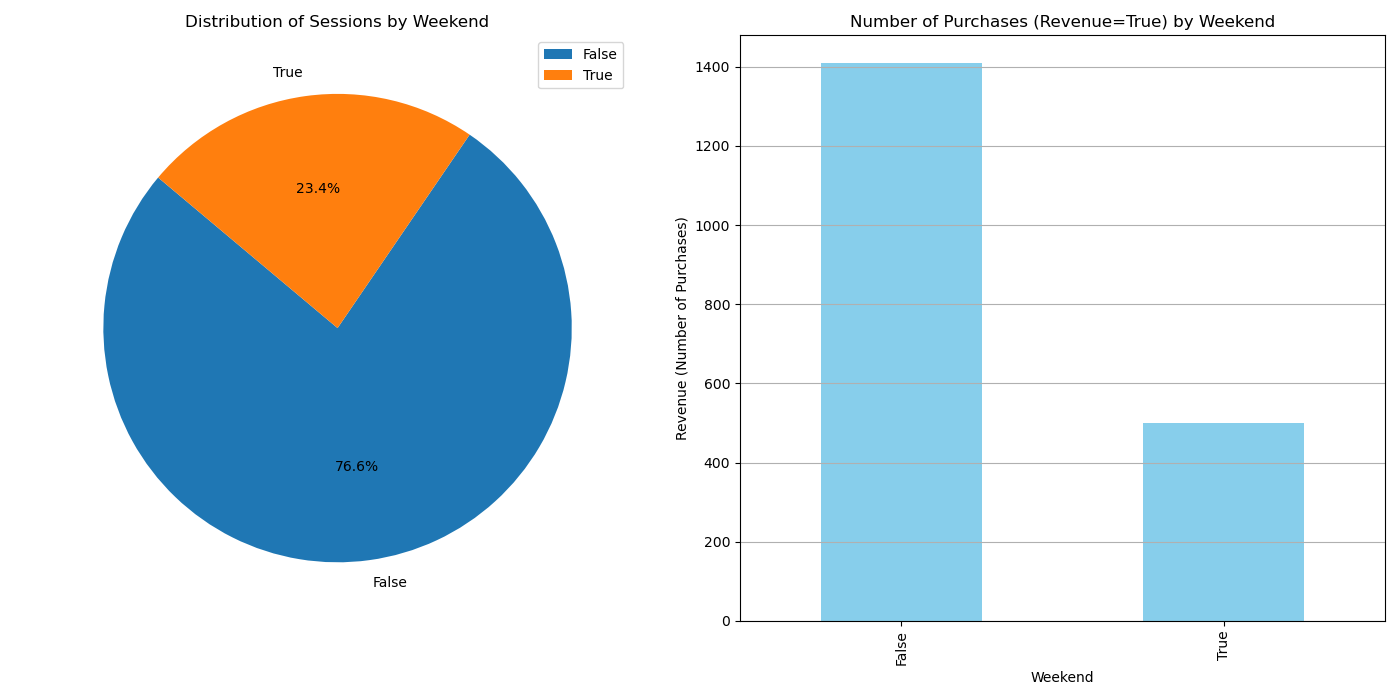
\includegraphics[width=0.8\textwidth,height=\textheight]{../results/figure_weekend_distribution.png}

}

\caption{\label{fig-weekend-distribution}Distribution of Sessions by
Weekend}

\end{figure}%

\paragraph{Continuous numerical Features: Correlation with
Revenue}\label{continuous-numerical-features-correlation-with-revenue}

The remaining features are continuous numerical features. In order to
understand their significance to the target feature, Revenue, we will
make a correlation plot. To do this, we will create a copy of the
original data, and modify it so that:

\begin{itemize}
\item
  Only the numerical features are kept
\item
  Revenue is represented as a numerical feature so that it can be
  compared with the other numerical features
\end{itemize}

\begin{figure}[H]

\centering{

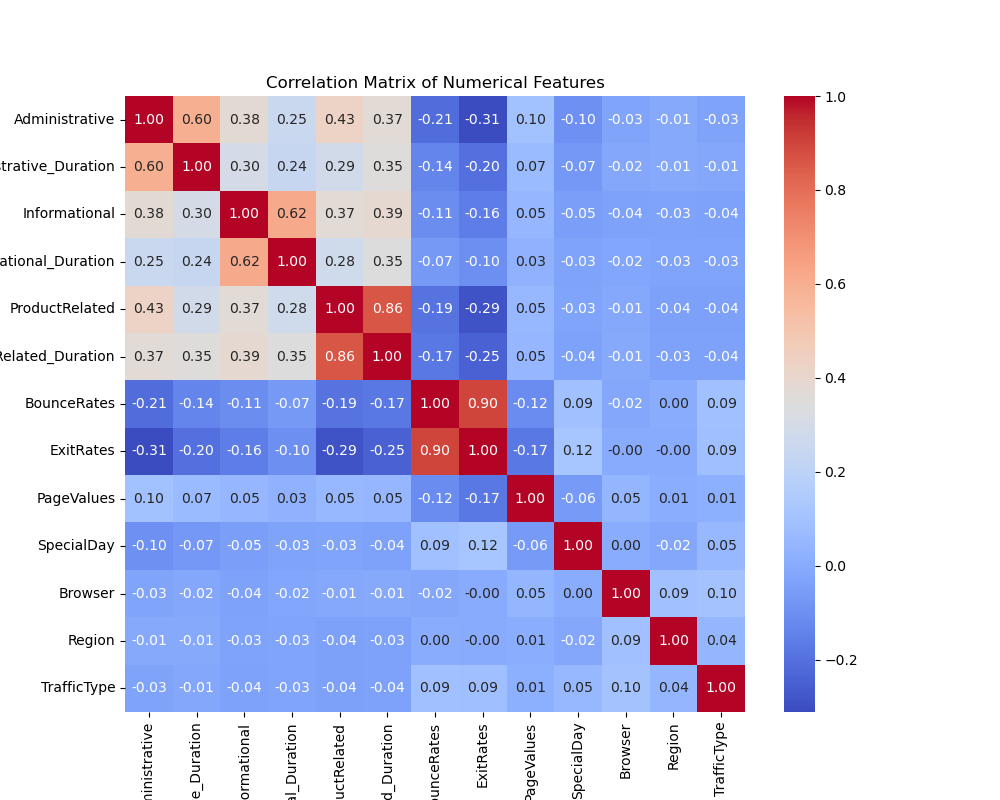
\includegraphics[width=0.8\textwidth,height=\textheight]{../results/figure_correlation_matrix.png}

}

\caption{\label{fig-corr\_matrix}Correlation Matrix of Numerical
Features}

\end{figure}%

From Figure~\ref{fig-corr_matrix}, we can see that the features most
strongly correlated with Revenue are: PageValues, ProductRelated, and
ProductRelated\_Duration. It is important to note that the correlation
matrix only represents linear correlations, between \emph{pairs} of
features. Some correlations may be confounded with other features, so
while this matrix is a good starting point, it may not capture all
relevant relationships.

\subsection{Methods}\label{methods}

\subsubsection{Analysis Plan}\label{analysis-plan}

\paragraph{1. Train-Test Split}\label{train-test-split}

Before applying any transformations or conducting any analysis, we will
first create a 70-30 split of our data:

\begin{itemize}
\item
  70\% split for the training subset
\item
  30\% split for the testing subset
\end{itemize}

All training of the models will be strictly conducted on the training
set. The testing set will only be used once the model is finalized, and
will only be deployed for scoring on the testing set once. This is to
ensure that the model is not exposed to the testing set so that it does
not `learn' off of what it is trying to predict.

\paragraph{2. Preprocessing and
Transformations}\label{preprocessing-and-transformations}

Given that we have different data types, we will apply some
transformations to each feature type depending on if the feature is
numerical and continuous, discrete and categorical, binary, etc. The
transformations will be detailed in Figure{[}INSERT LATER{]}.

\paragraph{3. Training Models}\label{training-models}

Our target feature, Revenue, is binary so the models chosen will be
trained to perform binary classification:

\textbf{3.1 Dummy Classifier Model}: The Dummy Classifier Model makes
predictions that ignore the input features, in other words, it does not
attempt to `learn' anything from the data. This classifier serves as a
baseline to compare to the following models.

\textbf{3.2 kNN:}

kNN is a simple cluster-based model. Given k, the number of nearest data
points, the kNN classifier takes a data point and classifies it
according to the the class of its k-nearest neighbours.

\textbf{3.3 SVM RBF:}

Support Vector Machines with RBF Kernels act as weighted KNN's. Unlike
KNN's, this model bases its decision boundary only on key examples,
known as support vectors. The model transforms the input features into a
higher dimensional space, generating a decision boundary based on a set
of positive and negative examples and their weights along with their
similarity measure. This model uses a kernel called RBFs as the
similarity metric.

\textbf{3.4 Random Forest Classifier:}

A Random Forest Classifier fits a series of decision tree classifiers on
subsets of the given data. Each tree `overfits' on a select feature,
however the model uses averaging of individual trees to improve the
predictive accuracy and therefore prevent overfitting. Given that there
are many features in our dataset, this model is a strong candidate for
our classification problem.

\subparagraph{Evaluating the models}\label{evaluating-the-models}

Each model will be evaluated on the following:

\begin{itemize}
\item
  fit time
\item
  score time
\item
  test score (this is the validation score, not the score from the
  actual test subset)
\item
  train score
\end{itemize}

The model with the best (validation) test score will then be deployed
\textbf{once} on the test data to obtain a final test score.

\subsubsection{Analysis}\label{analysis}

\subsubsection{1. Train Test Split}\label{train-test-split-1}

\textbf{Note}:

Before splitting the data, the feature Revenue will be transformed at
this step as it needs to be transformed to a numerical format using
one-hot encoding. This is done at this step because it will be removed
from the X\_train and X\_test sets.

\subsubsection{2. Preprocessing and
Transformations}\label{preprocessing-and-transformations-1}

\begin{longtable}[]{@{}
  >{\raggedright\arraybackslash}p{(\columnwidth - 4\tabcolsep) * \real{0.2653}}
  >{\raggedright\arraybackslash}p{(\columnwidth - 4\tabcolsep) * \real{0.4082}}
  >{\raggedright\arraybackslash}p{(\columnwidth - 4\tabcolsep) * \real{0.3265}}@{}}
\caption{Data Preprocessing
Summary}\label{tbl-preprocessing}\tabularnewline
\toprule\noalign{}
\begin{minipage}[b]{\linewidth}\raggedright
\textbf{Feature}
\end{minipage} & \begin{minipage}[b]{\linewidth}\raggedright
\textbf{Transformation}
\end{minipage} & \begin{minipage}[b]{\linewidth}\raggedright
\textbf{Explanation}
\end{minipage} \\
\midrule\noalign{}
\endfirsthead
\toprule\noalign{}
\begin{minipage}[b]{\linewidth}\raggedright
\textbf{Feature}
\end{minipage} & \begin{minipage}[b]{\linewidth}\raggedright
\textbf{Transformation}
\end{minipage} & \begin{minipage}[b]{\linewidth}\raggedright
\textbf{Explanation}
\end{minipage} \\
\midrule\noalign{}
\endhead
\bottomrule\noalign{}
\endlastfoot
Administrative & scaling & standardize scale with other numerical
features \\
Administrative\_Duration & scaling & standardize scale with other
numerical features \\
Informational & scaling & standardize scale with other numerical
features \\
Informational\_Duration & scaling & standardize scale with other
numerical features \\
ProductRelated & scaling & standardize scale with other numerical
features \\
ProductRelated\_Duration & scaling & standardize scale with other
numerical features \\
BounceRates & scaling & standardize scale with other numerical
features \\
ExitRates & scaling & standardize scale with other numerical features \\
PageValues & scaling & standardize scale with other numerical
features \\
SpecialDay & scaling & standardize scale with other numerical
features \\
Month & one-hot encoding & categorical feature, need a numerical
representation to pass through models \\
OperatingSystems & drop & justified in EDA, not relevant \\
Browser & n/a & would apply one-hot encoding but already represented in
numerical form \\
Region & n/a & would apply one-hot encoding but already represented in
numerical form \\
TrafficType & n/a & would apply one-hot encoding but already represented
in numerical form \\
VisitorType & one-hot encoding & categorical feature, need a numerical
representation to pass through models \\
Weekend & one-hot encoding with `binary=True' & categorical feature,
need a numerical representation to pass through models \\
\end{longtable}

The summary of preprocessing transformations and the explanation behind
each is provided in Table~\ref{tbl-preprocessing}.

\subsubsection{Training Models}\label{training-models-1}

For this analysis, we defined a custom function that returns the mean
and standard deviation cross validation scores. For each model, a
pipeline was defined to first preprocess the training split of the data,
then pass it through the model to be fit. The documentation of the
function is as follows:

\textbf{Parameters} * model :scikit-learn model * X\_train : numpy array
or pandas DataFrame * X in the training data * y\_train : * y in the
training data

\textbf{Returns} * pandas Series with mean scores from cross\_validation

\textbf{Note}: this function definition is taken from CPSC330 2023W1
Course Notes

Moreover, the results of each of the models described in the Analysis
Plan section is stored in a table to facilitate comparison of their fit
time, score time, test score, and train scores -- including the cross
validation scores for each metric.

\paragraph{Model Results}\label{model-results}

\begin{longtable}[]{@{}llllll@{}}
\toprule\noalign{}
& Unnamed: 0 & fit\_time & score\_time & test\_score & train\_score \\
\midrule\noalign{}
\endhead
\bottomrule\noalign{}
\endlastfoot
0 & Dummy & 0.006 (+/- 0.002) & 0.004 (+/- 0.001) & 0.847 (+/- 0.000) &
0.847 (+/- 0.000) \\
1 & KNN\_best\_k & 0.016 (+/- 0.007) & 1.324 (+/- 0.328) & 0.877 (+/-
0.005) & 0.880 (+/- 0.001) \\
2 & SVM\_RBF & 8.417 (+/- 1.140) & 2.303 (+/- 0.344) & 0.887 (+/- 0.002)
& 0.889 (+/- 0.000) \\
3 & Random\_Forest & 3.847 (+/- 0.409) & 0.090 (+/- 0.029) & 0.902 (+/-
0.004) & 1.000 (+/- 0.000) \\
\end{longtable}

\subsubsection{Model Selection}\label{model-selection}

Among the many factors that data scientists consider for model
selection, the two main factors we will consider are accuracy and
efficiency.

\paragraph{Efficiency}\label{efficiency}

Time efficiency and computational complexity are key factors to model
selection. We want models that strike the best balance between getting
the results we want and doing it in an efficient manner. KNN is known
for its computational intensity, although not reflected in the fit times
above, we can be concerned how it might performed on a larger scale.
Similarly, we know that the SVM model struggles with computational
efficiency and that is what our results reflected in the the fit time.
The random forests model came out on top of the efficiency tables with
the quickest fit time and scoring time while outperforming all other
models in terms of score as well.

\paragraph{Performance}\label{performance}

In assessing the accuracy of machine learning models, particularly in
the context of comparing Random Forests, kNN, and SVM, it's essential to
evaluate various metrics and considerations that provide an in-depth
evaluation truly reflective of performance. Each of these models offers
distinct approaches to classification and regression tasks, leading to
variations in performance across different datasets and problem domains.
In terms of our results, the clear winner is the random forest model.

\paragraph{Evaluating True Positive Rate, Precision
Score}\label{evaluating-true-positive-rate-precision-score}

The accuracy score at face value seems to be good, however if we break
down further our results by looking at our true positive rate (precision
score), we can see that our model actually struggled and because of the
class imbalance the effect of this on our score was not reflected in our
accuracy. This analysis helps us tame our optimism and helps us insights
into how well our model correctly identifies positive instances within
the dataset, which is particularly crucial in scenarios with imbalanced
classes. Understanding the nuances of class imbalances allows us to make
informed decisions about model adjustments, such as implementing
techniques like oversampling, undersampling, or adjusting class weights,
to improve the model's predictive capability for minority classes.
Moreover, it underscores the importance of considering multiple
evaluation metrics beyond just accuracy, enabling a more comprehensive
assessment of model effectiveness and guiding future iterations or
refinements to enhance predictive performance across all classes.

Figure~\ref{fig-rf_matrix} illustrates the distribution of the true
positives, false positives, true negatives, false negatives for the
Random Forests Model. This will be used to calculate the precision score
of the model.

\begin{figure}[H]

\centering{

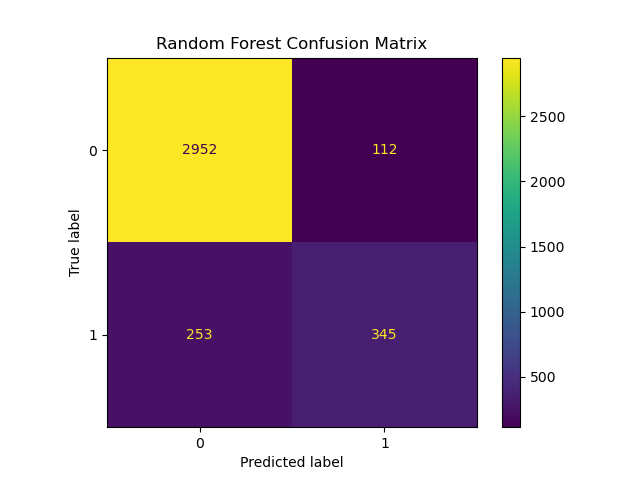
\includegraphics[width=0.8\textwidth,height=\textheight]{../results/random_forest_confusion_matrix.png}

}

\caption{\label{fig-rf\_matrix}Random Forests Confusion Matrix}

\end{figure}%

To obtain the precision score of our model, the following formula was
used:

\[ s = TP / (TP + FP) \]

Given this formula, the precision score is: Precision = 0.5585.

\paragraph{Conclusion}\label{conclusion}

Our findings can be summed up into 2 main points:

When it comes to the application of ML to predict online consumer
behaviour, the random forests model performs the best and produced the
best results.

Random forests was both efficient and accurate. The results provided a
very simple solution without much to be further analyzed.

\subparagraph{Margin For Error}\label{margin-for-error}

Our results are purely based on the models that we chose to test, and
therefore, may not be the absolute best off the shelf models for the
given project but in favour of simplicity and the essence of time, among
the 3 tested models (KNN, SVM and RF), we've concluded that the random
forests model performed the best.

While it was the best-performing model, the final model's precision
score of 56\% indicates that the model only predicts the positive class
correctly roughly half the time. This could be indicative that the model
was quite overfitted on the training model, or that despite the
randomization of our train-test split, the training sample was not a
good representation of the test split and perhaps the true population of
online shoppers sampled in our dataset. Likely, the low precision score
is highly influenced by the fact that there was class imbalance in our
dataset, as demonstrated in Figure~\ref{fig-revenue-distribution}, which
shows that there are over 4 times more false cases than true for the
feature Revenue. As a consequence, the models, no matter how well they
perform on the training dataset, are bound to better learn the
predictive features for a false Revenue case than a true revenue case
simply because of the class distribution in the original dataset.

For future analysis, perhaps the class imbalance may be addressed by
selectively sampling to have fair distribution of both Revenue classes,
rather than pure random sampling as was done in our analysis.

\subsection*{References}\label{references}
\addcontentsline{toc}{subsection}{References}

\phantomsection\label{refs}
\begin{CSLReferences}{1}{0}
\bibitem[\citeproctext]{ref-Gkikas2022}
Gkikas, Dimitris C., and Prokopis K. Theodoridis. 2022. {``AI in
Consumer Behavior.''} In \emph{Advances in Artificial Intelligence-Based
Technologies: Selected Papers in Honour of Professor Nikolaos g.
Bourbakis---Vol. 1}, edited by Maria Virvou, George A. Tsihrintzis,
Lefteri H. Tsoukalas, and Lakhmi C. Jain, 147--76. Cham: Springer
International Publishing.
\url{https://doi.org/10.1007/978-3-030-80571-5_10}.

\bibitem[\citeproctext]{ref-Monteros_2023}
Monteros, Maria. 2023. {``Big-Box Retailers Continue to Ramp up
Investments in Store-Based Fulfillment.''} \emph{Modern Retail}.
\url{https://www.modernretail.co/operations/big-box-retailers-continue-to-ramp-up-investments-in-store-based-fulfillment/}.

\bibitem[\citeproctext]{ref-Sakar_Polat_Katircioglu_Kastro_2018}
Sakar, C. Okan, S. Olcay Polat, Mete Katircioglu, and Yomi Kastro. 2018.
{``Real-Time Prediction of Online Shoppers' Purchasing Intention Using
Multilayer Perceptron and LSTM Recurrent Neural Networks.''}
\emph{Neural Computing and Applications} 31 (10): 6893--6908.
\url{https://doi.org/10.1007/s00521-018-3523-0}.

\bibitem[\citeproctext]{ref-Shaw_Eschenbrenner_Baier_2022}
Shaw, Norman, Brenda Eschenbrenner, and Daniel Baier. 2022. {``Online
Shopping Continuance After COVID-19: A Comparison of Canada, Germany and
the United States.''} \emph{Journal of Retailing and Consumer Services}
69 (November): 103100.
\url{https://doi.org/10.1016/j.jretconser.2022.103100}.

\end{CSLReferences}



\end{document}
